\documentclass{article}
\usepackage{graphicx} % Required for inserting images
\usepackage[table,xcdraw]{xcolor}
\usepackage{authblk}
\usepackage{hyperref}
\usepackage{listings}
\usepackage{xcolor}
\usepackage{caption}
\usepackage{graphicx}
\usepackage{subcaption}
\usepackage{grffile}
\usepackage{pdfpages}
\usepackage{float}
\usepackage{booktabs}
\usepackage{multirow}
\captionsetup[lstlisting]{labelformat=empty}
\captionsetup[table]{labelformat=empty}
\captionsetup[figure]{labelformat=empty}
\captionsetup[subfigure]{labelformat=empty}
\usepackage[a4paper, left=2cm, right=2cm, top=2.3cm, bottom=2.3cm]{geometry}
\usepackage{csvsimple}
\usepackage[utf8]{inputenc}
\usepackage{csquotes}
\usepackage[backend=biber,style=apa]{biblatex}
\usepackage[spanish]{babel}
\usepackage{float}

\addbibresource{referencias.bib} % Vincula el archivo .bib

\title{Detección de cáncer de pulmón con un enfoque basado en aprendizaje automático y aprendizaje profundo}
\author[1]{Abarca Cruz Zdenko Emilio}
\author[2]{Aburto Lopéz Francisco Javier}
\author[3]{Fuentes Herrera Carlos}
\author[4]{Ramírez Rodríguez Enrique}
\affil[1]{Ingeniería en Computación, Universidad Autónoma del Estado de México}
\affil[2]{Matemáticas Aplicadas y Computación, Facultad de Estudios Superiores Acatlán}
\affil[3]{Ingeniería en Mecatrónica, Unidad profesional Interdisciplinaria en Ingeniería y Tecnologías Avanzadas IPN}
\affil[4]{Matemáticas Aplicadas y Computación, Facultad de Estudios Superiores Acatlán}
\addbibresource{referencias.bib} % Vincula el archivo .bib
\begin{document}

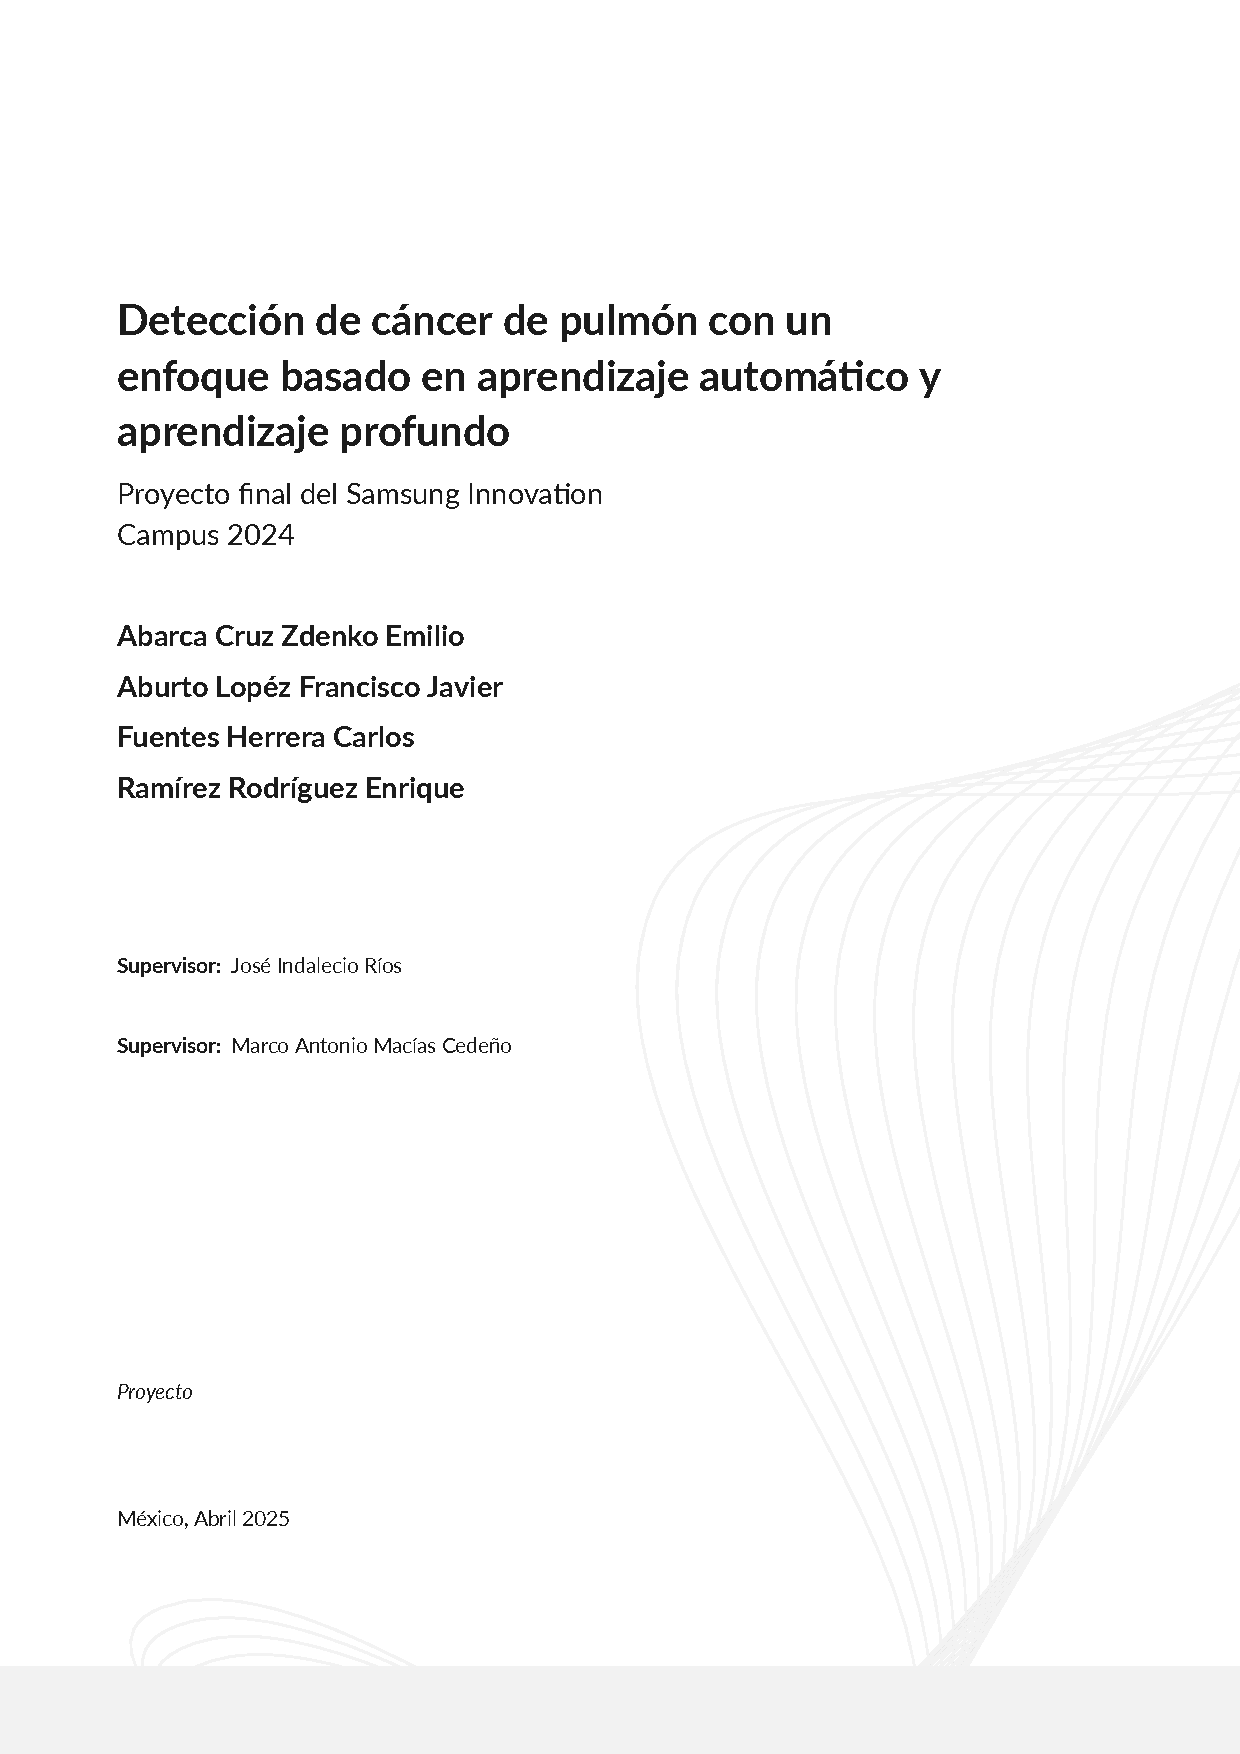
\includepdf{Portada_SIC.pdf}

% z\maketitle

\newpage

\tableofcontents

\newpage

\section{Introducción}
    % Introducción
 % \chapter{Introducción}
El presente proyecto se desarrolla como parte del curso de \textbf{Samsung Innovation Campus} sobre \textbf{Inteligencia Artificial y Liderazgo}. El objetivo es aplicar los conocimientos adquiridos en el diseño e implementación de modelos de IA en una problemática específica, generando información de utilidad y explorando la capacidad de la inteligencia artificial para resolver problemas reales o crear soluciones innovadoras.

La \textbf{temática elegida} fue el cáncer de pulmón, una de las principales causas de muerte en el mundo (\cite{WHO2025}). Su diagnóstico temprano es fundamental, ya que permite un tratamiento más efectivo y reduce los costos médicos al evitar intervenciones complejas en etapas avanzadas. Sin embargo, la detección temprana presenta desafíos significativos, como la falta de acceso a especialistas en algunas regiones y la complejidad de interpretar imágenes médicas \parencite{OMS2017diagnosis}.

% Síntomas

Según \textcite{MNT2025}, el cáncer de pulmón puede causar varios síntomas que pueden indicar que existe un problema en los pulmones.
Entre los síntomas más comunes se encuentran los siguientes:

\begin{itemize}
    \item Tos persistente
    \item Dolor torácico
    \item Disnea
    \item Tos con sangre (hemoptisis)
    \item Cansancio
    \item Pérdida de peso inexplicada
    \item Infecciones pulmonares recurrentes
\end{itemize}

% Pronóstico

El pronóstico del cáncer de pulmón depende de múltiples factores como el tipo de cáncer, el estadio en el momento del diagnóstico, la edad y salud general del paciente. Según datos de la Sociedad Americana Contra el Cáncer\parencite{ACS2025}, la tasa de supervivencia a 5 años varía significativamente dependiendo del tipo de cáncer y de la etapa en la que se diagnostique, siendo mayor cuando se detecta en etapas tempranas.

\begin{table}[h!]
\centering
\begin{tabular}{|c|c|c|}
\hline
Etapa & CPCNP & CPCP \\
\hline
%\rowcolor[HTML]{FFD700}   % Color de fondo alternado
Localizado(aún en la ubicación original) & 63 por ciento & 27 por ciento \\
\hline
Regional(Se ha extendido a zonas cercanas)& 35 por ciento & 16 por ciento \\
\hline
%\rowcolor[HTML]{D3D3D3 }  % Color de fondo alternado
Distante o metastásica(Se ha diseminado por todo el cuerpo)& 7 por ciento & 3 por ciento \\
\hline
General & 25 por ciento & 7 por ciento \\
\hline
\end{tabular}
\caption{Supervivencia según etapa y tipo de cáncer de pulmón.}
\end{table}

% Diagnóstico

El diagnóstico del cáncer de pulmón se basa en una combinación de estudios que incluyen exploraciones físicas, imágenes médicas (radiografías, tomografías computarizadas y resonancias magnéticas), broncoscopias, biopsias y pruebas moleculares para identificar mutaciones genéticas específicas. Estos procedimientos permiten determinar la etapa del cáncer y guiar el tratamiento.

% Problemática
\subsection{Problematica}
El cáncer de pulmón es la principal causa de muertes relacionadas con el cáncer a nivel mundial, siendo responsable de aproximadamente el 85\% de los casos debido al tabaquismo\parencite{WHO2025}. Este cáncer se diagnostica frecuentemente en etapas avanzadas, lo que limita las opciones de tratamiento y reduce las probabilidades de supervivencia.

Además, la detección oportuna se ve obstaculizada por la falta de acceso a tecnologías avanzadas de diagnóstico, la carencia de especialistas en áreas rurales y la complejidad de interpretar imágenes médicas de manera precisa. Esto resalta la necesidad de desarrollar herramientas que faciliten el diagnóstico temprano y preciso, disminuyendo la mortalidad asociada al cáncer de pulmón\parencite{mayoclinic_lung_cancer}.

Los tipos más comunes de cáncer de pulmón son el carcinoma no microcrítico (NSCLC) y el carcinoma microcrítico (SCLC). El NSCLC es más común y crece lentamente, mientras que el SCLC es menos común pero de crecimiento rápido\parencite{WHO2025}.

% Datos Mundiales 
\subsection{Datos a Nivel Mundial}
Según la Sociedad Americana Contra el Cáncer\parencite{cancer_american}, para el año 2025 se estiman los siguientes datos en Estados Unidos:
\begin{itemize}
    \item 226,650 nuevos casos de cáncer de pulmón.
    \item 124,730 muertes por cáncer de pulmón.
\end{itemize}
A nivel mundial, el cáncer de pulmón representa el 12.4\% de todos los diagnósticos de cáncer, con aproximadamente 2.21 millones de casos nuevos diagnosticados en 2022. Además, es la principal causa de muerte por cáncer, responsable del 18.7\% de las muertes por cáncer, con alrededor de 1.8 millones de muertes anuales. Este cáncer afecta principalmente a personas mayores de 65 años y se asocia principalmente con factores de riesgo como el tabaquismo, que es responsable del 85\% de los casos, así como la exposición a sustancias tóxicas y la contaminación ambiental \parencite{anticancerlifestyle,cancerorg,who}
%Datos en México
\subsection{Datos en México}
En México, el cáncer de pulmón es la causa más letal entre los tipos de cáncer, con más de 8,000 muertes al año (\cite{INCan2025}). En 2018 se reportaron más de 9,000 nuevos casos, de los cuales el 85\% estaban relacionados con el tabaquismo. A pesar de los esfuerzos por mejorar el diagnóstico, la detección en etapas avanzadas sigue siendo un problema.

% Justificación
\subsection{Justificación}
Este proyecto se desarrolla como parte del curso de Samsung Innovation Campus sobre Inteligencia Artificial y Liderazgo. Se busca aplicar los conocimientos adquiridos en el diseño e implementación de modelos de IA en una problemática específica que sea capaz de generar información de utilidad.

A través de este trabajo, se busca aplicar conceptos teóricos y prácticos aprendidos durante el curso, explorando la capacidad de los modelos de IA para resolver problemas reales o crear soluciones innovadoras.

La selección de la temática fue completamente libre, el tema que decidimos a tratar fue cáncer de pulmón, debido a que es una de las principales causas de muerte en el mundo, con una alta tasa de mortalidad y su detección temprana podría salvar miles de vidas al permitir tratamientos más efectivos y a su vez reducir los costos de tratamiento, esto contribuiría a reducir la mortalidad asociada a la enfermedad y a optimizar los recursos médicos, ofreciendo una herramienta accesible y de gran impacto social.

Este proyecto no solo permitirá aplicar conocimientos técnicos, sino que también representa una oportunidad para explorar el impacto positivo de la IA en el campo de la salud, alineándose con los objetivos del Samsung Innovation Campus de fomentar el desarrollo de habilidades tecnológicas con un enfoque práctico y transformador.\\

% Objetivos

\subsection{Objetivo General}
Desarrollar un modelo de inteligencia artificial capaz de diagnosticar el cáncer de pulmón de manera temprana y precisa, contribuyendo a reducir la tasa de mortalidad y optimizando el tratamiento médico.\\
\subsection{Objetivos Específicos}
\begin{itemize}
    \item Desarrollar un modelo de IA capaz de detectar el cáncer de pulmón en etapas tempranas, facilitando el diagnóstico oportuno y mejorando las probabilidades de tratamiento efectivo.
    \item Búsqueda de bases de datos open source.
    \item Análisis sistemático de literatura 
    \item Desarrollar un proceso estandarizado para la extracción y procesamiento de datos relevantes de las bases de datos seleccionadas.
    \item  Aplicar conceptos teóricos y prácticos aprendidos durante el curso, explorando la capacidad de los modelos de IA.
    \item Identificar patrones complejos y sutiles en imágenes médicas mediante técnicas avanzadas de procesamiento de imágenes.
\end{itemize}

% Revision de literatura

\subsection{Revisión de Literatura: Aplicaciones de la Inteligencia Artificial en la Predicción y Diagnóstico del Cáncer de Pulmón}
La inteligencia artificial (IA) ha emergido como una herramienta revolucionaria en el campo de la salud, permitiendo diagnósticos más precisos, pronósticos personalizados y tratamientos optimizados para diversas enfermedades, incluido el cáncer de pulmón. A continuación, se presentan algunas de las aplicaciones más destacadas de la IA en el manejo del cáncer de pulmón:

\begin{itemize}
    \item \textbf{Redes Neuronales Convolucionales (CNNs):}En el estudio de Hatuwal y Thapa (2020) titulado "Lung Cancer Detection Using Convolutional Neural Network on Histopathological Images", publicado en el International Journal of Computer Trends and Technology\parencite{CNN1}, se utilizó una red neuronal convolucional (CNN) para detectar el cáncer de pulmón a partir de imágenes histopatológicas. Este tipo de imágenes son esenciales en el diagnóstico del cáncer, ya que proporcionan detalles a nivel celular sobre los tejidos afectados, se pueden ver los resultados en la sección conclusión.

    El articulo "Deep Learning for Computer Vision: A Brief Review" proporciona una revisión general sobre cómo el aprendizaje profundo (Deep Learning) ha revolucionado el campo de la visión por computadora (Computer Vision). En particular, cubre los avances en redes neuronales convolucionales (CNNs) y otras arquitecturas de redes profundas que se han aplicado exitosamente en tareas como clasificación de imágenes, detección de objetos, y segmentación de imágenes, entre otras, los resultados se pueden observar en la conclusión \parencite{CNN2}.
    
    \item\textbf{XGBClassifier}El artículo "Lung and colon cancer classification using medical imaging: a feature engineering approach" ,(2022) presenta un sistema asistido por computadora para clasificar de manera precisa tejidos de cáncer de colon y pulmón utilizando imágenes histopatológicas. El estudio aplica técnicas de aprendizaje automático y procesamiento de imágenes, utilizando modelos como XGBoost \parencite{modelo_XGBClassifier}, se pueden ver los resultados del estudio en la sección conclusión.


\end{itemize}

Una de las aplicaciones más innovadoras de la IA es el análisis histopatológico de imágenes de biopsias teñidas con hematoxilina y eosina (H\&E). Esta técnica ha permitido a los sistemas de IA identificar y cuantificar patrones complejos que serían difíciles de detectar manualmente. Un estudio publicado en \textit{Nature Communications} presentó \textbf{SEQUOIA}, una herramienta de IA capaz de predecir la actividad de miles de genes en células tumorales utilizando solo imágenes de biopsias teñidas con H\&E. Los resultados mostraron una correlación superior al 80\% entre las predicciones de la IA y los datos reales de actividad genética en tipos específicos de cáncer \parencite{labmedica2025}.

El análisis histopatológico automatizado no solo permite detectar células tumorales, sino que también cuantifica la densidad celular y calcula índices de proliferación, lo que facilita la estratificación de pacientes según el riesgo y la personalización de tratamientos oncológicos. Esta tecnología puede clasificar imágenes con una precisión sorprendente, lo que agiliza la toma de decisiones clínicas y reduce el tiempo diagnóstico \parencite{roche2025}.

Además, el enfoque interdisciplinario de la IA y las biopsias digitales ha abierto nuevas oportunidades para la investigación clínica, permitiendo explorar correlaciones entre patrones histológicos y resultados clínicos. Esto no solo mejora el diagnóstico y el pronóstico del cáncer de pulmón, sino que también proporciona un marco más robusto para desarrollar nuevas terapias dirigidas y medicina personalizada \parencite{labmedica2025}.

En resumen, la integración de la inteligencia artificial en el diagnóstico y tratamiento del cáncer de pulmón ha permitido avances significativos en la detección temprana, el pronóstico preciso y la planificación terapéutica personalizada. Estos enfoques innovadores continúan evolucionando, prometiendo un futuro en el que la IA desempeñe un papel cada vez más crucial en la lucha contra el cáncer de pulmón.

\subsection{Entrevista con el Dr. Alberto Daniel Saucedo Campos  - ISSTE}

Se realizó una entrevista con el Dr. Alberto Daniel Saucedo Campos, especialista en oncología del ISSSTE, para conocer su perspectiva sobre el diagnóstico y seguimiento de cancer de pulmón mediante herramientas de inteligencia artificial con el objetivo de conocer su perspectiva sobre la detección temprana de neoplasias mediante el uso de modelos basados en inteligencia artificial.

\textbf{Preguntas y respuestas:}
\begin{itemize}
\item \textbf{¿Cuáles son las principales dificultades para diagnosticar cancer de pulmón?}
\textit{El problema del cáncer de pulmón es que en sus etapas iniciales no da síntomas, no duele, no provoca sangrados a veces puede provocar una tos muy leve que se puede confundir con una alergia, una gripa, infortunadamente el cáncer de pulmón hasta que llega a niveles de invasión del bronquio más intenso es cuando se comienza con la disnea y mínimo puede que ya este en la etapa 3. Entonces ese es el problema principalmente, que las neoplasias son muy silenciosas}
\item\textbf{¿Qué tipo de errores diagnósticos son más comunes en la práctica clínica? }
\textit{El cáncer es una enfermedad muy catastrófica, si vemos la cantidad de diabéticos, de hipertensos que tenemos vs los que tienen cáncer, pues la proporción que tenemos es de 30 a 1, por cada 30 diabéticos va a haber uno con cáncer, entonces infortunadamente el clínico no piensa de primera intención en cáncer, hasta que les hacen la placa, y típicamente cuando hacen la placa encuentran una cosa que se llama nódulo solitario, es cuando comienzan a sospechar de que puede ser una neoplasia. Actualmente lo que se está haciendo es buscar marcadores moleculares en sangre cuando haya la sospecha, y pues ahí en lo que se enfoca principalmente es en la historia clínica, si el paciente es fumador, si está expuesto a biomasas, es decir, que tenga contacto con anafres, con polvos intensos, humos, ya que es importante en la historia clinica.}
\item\textbf{¿Qué papel juega el médico de primer contacto en el diagnóstico inicial?}
\textit{El médico de primer contacto juega un papel importante ya que debe realizar un diagnóstico preliminar basado en los síntomas del paciente y muchas veces no tienen la preparación para sospecharlo y cuando lo sospechan no saben qué buscar.}
\item \textbf{¿Cómo podría un sistema predictivo mejorar el diagnóstico?}
\textit{Un modelo de predicción con inteligencia artificial puede identificar factores de riesgo y calcular la probabilidad de enfermedad antes de que los síntomas se presenten, permitiendo un seguimiento médico más eficiente.}
\item \textbf{¿Cómo ve el uso de modelos predictivos para seguimiento de pacientes?}
\textit{Podrían reducir costos, optimizar recursos y permitir un monitoreo constante, especialmente en pacientes de alto riesgo.}
\item \textbf{¿Qué aspectos clave deben considerarse al implementar un sistema de predicción de enfermedades?}
\textit{La precisión del modelo, la accesibilidad y el acompañamiento médico para interpretar los resultados.}
\end{itemize}


En la entrevista, se discutieron las principales dificultades para diagnosticar el cáncer de pulmón, enfatizando que la enfermedad suele ser asintomática en etapas tempranas, lo que dificulta una detección oportuna. Frecuentemente, los síntomas iniciales son leves y se confunden con afecciones menores, lo que retrasa el diagnóstico hasta etapas avanzadas.

El doctor destacó que en la práctica clínica, el diagnóstico temprano del cáncer de pulmón es complejo debido a que los médicos de primer contacto no suelen considerarlo inicialmente. Este error diagnóstico es común, ya que se priorizan enfermedades más frecuentes como la diabetes o la hipertensión. Por lo general, el cáncer de pulmón solo se sospecha tras realizar una radiografía que revela un nódulo solitario. En respuesta a esta problemática, se mencionó que actualmente se buscan marcadores moleculares en sangre para una detección más precisa cuando hay sospechas fundadas, además de realizar una historia clínica exhaustiva enfocada en factores de riesgo como el tabaquismo y la exposición a biomasas y polvos intensos.

Respecto al papel del médico de primer contacto, el doctor señaló que su intervención es fundamental para un diagnóstico temprano, aunque la falta de preparación específica limita su capacidad de identificar la enfermedad.

Finalmente, el doctor expresó que un modelo de predicción basado en inteligencia artificial (IA) podría transformar el diagnóstico y seguimiento de pacientes con cáncer de pulmón al calcular el riesgo antes de la aparición de síntomas. Este enfoque permitiría optimizar recursos, reducir costos y ofrecer un monitoreo constante a pacientes de alto riesgo. No obstante, enfatizó que la precisión del modelo, la accesibilidad y el acompañamiento médico adecuado son aspectos críticos para la implementación exitosa de esta tecnología



\newpage



\newpage
\newpage

% Problematica, justificación, general, objetivos especíwficos

\section{Metodología}
 
    \subsection{Metodología de clasificación}
        Para trabajar con el problema de agrupamiento se utilizó el \textit{datset} ``Lung Cancer Prediction'', que puede consultarse en la página de Kaggle. Dicho \textit{dataset} tiene  mil registros de pacientes con cáncer de pulmón, cuenta con  25 características, entre las que se encuentran; edad, género, contaminación del aire, riesgo genético, dolor de pecho y el nivel de su condición (bajo, medio y alto). Si bien esta última característica podría permitirnos considerar a los datos como etiquetados, no la tomaremos en cuenta para poder trabajarlos con métodos de aprendizaje no supervisado. 

Las versiones de \textit{Python} y las librerías utilizadas fueron las siguientes:
\begin{itemize}
	\item  Pandas versión: 2.2.2
	
	\item  NumPy versión: 2.0.2
	
	\item  Seaborn versión: 0.13.2
	
	\item  Matplotlib versión: 3.10.0
	
	\item Sklearn versión: 1.6.1
	
	\item SciPy versión: 1.14.1
\end{itemize}

Como ya se mencionó, los registros tienen la característica \textit{'Level'}, por lo que el objetivo de esta sección es implementar métodos de agrupamiento para generar 3 \textit{clústeres} que nos permitan agrupar nuestros de manera similar a la característica \textit{'Level'}, debido a esto utilizaremos métodos de no jerárquicos, posteriormente utilizaremos el método \textit{PCA} para reducir la dimensión de nuestra \textit{dataset} para poder visualizar los \textit{clústeres} generados en gráficos 2D y 3D, finalmente compararemos los resultados que obtuvimos del agrupamiento con los datos originales para conocer la precisión que obtuvimos.

Primero hacemos una copia del \textit{dataset} con el que estamos trabajando y eliminamos las características \textit{'index', 'Patient ID'} y \textit{'Level'}, pues las primeras dos no son relevantes para el agrupamiento y ya planteamos que la última la usaremos para conocer la precisión que obtuvimos.

\subsubsection{Agrupamiento con k-means}

\lstset{
    language=Python,
    basicstyle=\ttfamily\footnotesize,
    keywordstyle=\color{blue},
    commentstyle=\color{gray},
    stringstyle=\color{green!60!black},
    numberstyle=\tiny\color{gray},
    numbers=left,
    breaklines=true,
    frame=single,
    captionpos=b,
    tabsize=4,
    showspaces=false,
    showstringspaces=false,
    showtabs=false
}
		
\begin{lstlisting}
    cancer_data = df.drop(columns=["Patient Id", "Level", "index"])

    # Estandarizamos los datos 
    scaler = StandardScaler()
    scaled_data = scaler.fit_transform(cancer_data)

    # Los convertimos en una data frame
    scaled_data_df = pd.DataFrame(scaled_data, columns=cancer_data.columns)
\end{lstlisting}

\begin{lstlisting}[caption={Código de k-means}]
    # posibles grupos: Low, Medium y High
    kmeans = KMeans(n_clusters=3, random_state=42, n_init=10)
    kmeans.fit(scaled_data)

    scaled_data_df['cluster'] = kmeans.labels_
\end{lstlisting}

Hacemos una reducción de dimensiones para poder visualizar los datos en 2D y 3D.  

\begin{lstlisting}[caption={PCA para 2D}]
    pca = PCA(n_components=2)
    cancer_pca = pca.fit_transform(scaled_data)
    print(f"Varianza total explicada: {sum(pca.explained_variance_ratio_)*100:.2f}%")
\end{lstlisting}

\begin{lstlisting}[caption={PCA para 3D}]
    pca3 = PCA(n_components=3)
    cancer_pca3 = pca.fit_transform(scaled_data)
    print(f"Varianza total explicada: {sum(pca3.explained_variance_ratio_)*100:.2f}%")
\end{lstlisting}

\begin{figure}[!ht]
    \centering
    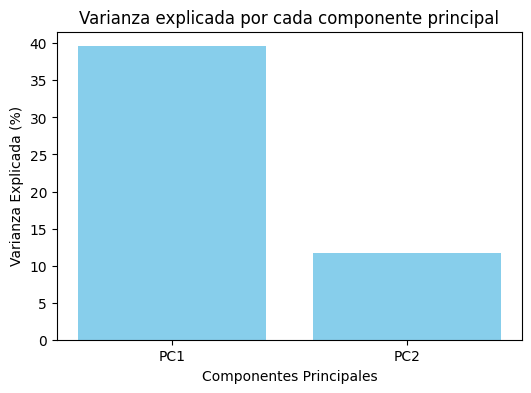
\includegraphics[scale = 0.75]{Enrique/Imagenes/Varianza_2d.png}
    \caption{Varianza de 51.32\%}
\end{figure}

\begin{figure}[!ht]
    \centering
    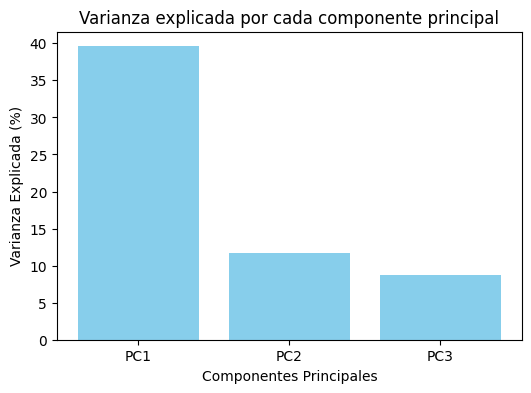
\includegraphics[scale = 0.75]{Enrique/Imagenes/varianza_3d.png}
    \caption{Varianza de 60.09\%}
\end{figure}

\subsubsection{Agrupamiento con DBSCAN}

También implementaremos el agrupamiento con el método \textit{DBSCAN}. Los primeros valores que proponemos para $\varepsilon$ y el número mínimo de muestras son 0.5 y 20 respectivamente, de lo cual obtenemos.

\begin{lstlisting}[caption={DSCAN con $\varepsilon$=0.5}]
    from sklearn.cluster import DBSCAN

    dbscan = DBSCAN(eps=.5, min_samples=20)
    dbscan.fit(scaled_data)

    print(dbscan.labels_.min(), dbscan.labels_.max())
\end{lstlisting}

\begin{lstlisting}[caption={Salida del código}]
    -1  9 
\end{lstlisting}

El -1 nos indica que el algoritmo clasificó algunos datos como \textit{atípicos}, que la etiqueta más grande sea 9 quiere decir que el algoritmo formó 10 grupos, como solo queremos formar 3 grupos, correremos el algoritmo para distintos valores de $\varepsilon$ hasta que solo se formen 3 \textit{clústeres}.

\begin{lstlisting}
    i = 0.5
    
    while dbscan.labels_.max() > 2:
        i += 0.1
        dbscan = DBSCAN(eps=i, min_samples=20)
        dbscan.fit(scaled_data)
        print(i, dbscan.labels_.min(), dbscan.labels_.max())
\end{lstlisting}

Con esto encontramos que la $\varepsilon$ que nos permite tener 3 grupos es 4.7, pero el algoritmo sigue clasificando algunos datos como atípicos, por lo que De manera similar encontramos el número de puntos mínimos

\begin{lstlisting}
    j = 20
    
    while dbscan.labels_.min() < 0 :
        j -= 1
        dbscan = DBSCAN(eps=4.9, min_samples=j)
        dbscan.fit(scaled_data)
        print(j, dbscan.labels_.min(), dbscan.labels_.max())
\end{lstlisting}

Finalmente obtenemos que $\varepsilon  =4.9$ y \textit{min\_samples = 19}, por lo que utilizaremos estos parámetros para el método \textit{DBSCAN}. Las etiquetas que obtengamos las guardaremos en una columna del \textit{dataframe scaled\_data\_df}

\begin{lstlisting}
    dbscan = DBSCAN(eps=4.9, min_samples=19)
    dbscan.fit(scaled_data)

    scaled_data_df['cluster DBSCAN'] = dbscan.labels_
\end{lstlisting}

\newpage
  
    \subsection{Metodología de predicción}    
        Para trabajar con el problema de agrupamiento se utilizó el \textit{datset} ``Lung Cancer Prediction'', que puede consultarse en la página de Kaggle. Dicho \textit{dataset} tiene  mil registros de pacientes con cáncer de pulmón, cuenta con  25 características, entre las que se encuentran; edad, género, contaminación del aire, riesgo genético, dolor de pecho y el nivel de su condición (bajo, medio y alto). Si bien esta última característica podría permitirnos considerar a los datos como etiquetados, no la tomaremos en cuenta para poder trabajarlos con métodos de aprendizaje no supervisado. 

Las versiones de \textit{Python} y las librerías utilizadas fueron las siguientes:
\begin{itemize}
	\item  Pandas versión: 2.2.2
	
	\item  NumPy versión: 2.0.2
	
	\item  Seaborn versión: 0.13.2
	
	\item  Matplotlib versión: 3.10.0
	
	\item Sklearn versión: 1.6.1
	
	\item SciPy versión: 1.14.1
\end{itemize}

Como ya se mencionó, los registros tienen la característica \textit{'Level'}, por lo que el objetivo de esta sección es implementar métodos de agrupamiento para generar 3 \textit{clústeres} que nos permitan agrupar nuestros de manera similar a la característica \textit{'Level'}, debido a esto utilizaremos métodos de no jerárquicos, posteriormente utilizaremos el método \textit{PCA} para reducir la dimensión de nuestra \textit{dataset} para poder visualizar los \textit{clústeres} generados en gráficos 2D y 3D, finalmente compararemos los resultados que obtuvimos del agrupamiento con los datos originales para conocer la precisión que obtuvimos.

Primero hacemos una copia del \textit{dataset} con el que estamos trabajando y eliminamos las características \textit{'index', 'Patient ID'} y \textit{'Level'}, pues las primeras dos no son relevantes para el agrupamiento y ya planteamos que la última la usaremos para conocer la precisión que obtuvimos.

\subsubsection{Agrupamiento con k-means}

\lstset{
    language=Python,
    basicstyle=\ttfamily\footnotesize,
    keywordstyle=\color{blue},
    commentstyle=\color{gray},
    stringstyle=\color{green!60!black},
    numberstyle=\tiny\color{gray},
    numbers=left,
    breaklines=true,
    frame=single,
    captionpos=b,
    tabsize=4,
    showspaces=false,
    showstringspaces=false,
    showtabs=false
}
		
\begin{lstlisting}
    cancer_data = df.drop(columns=["Patient Id", "Level", "index"])

    # Estandarizamos los datos 
    scaler = StandardScaler()
    scaled_data = scaler.fit_transform(cancer_data)

    # Los convertimos en una data frame
    scaled_data_df = pd.DataFrame(scaled_data, columns=cancer_data.columns)
\end{lstlisting}

\begin{lstlisting}[caption={Código de k-means}]
    # posibles grupos: Low, Medium y High
    kmeans = KMeans(n_clusters=3, random_state=42, n_init=10)
    kmeans.fit(scaled_data)

    scaled_data_df['cluster'] = kmeans.labels_
\end{lstlisting}

Hacemos una reducción de dimensiones para poder visualizar los datos en 2D y 3D.  

\begin{lstlisting}[caption={PCA para 2D}]
    pca = PCA(n_components=2)
    cancer_pca = pca.fit_transform(scaled_data)
    print(f"Varianza total explicada: {sum(pca.explained_variance_ratio_)*100:.2f}%")
\end{lstlisting}

\begin{lstlisting}[caption={PCA para 3D}]
    pca3 = PCA(n_components=3)
    cancer_pca3 = pca.fit_transform(scaled_data)
    print(f"Varianza total explicada: {sum(pca3.explained_variance_ratio_)*100:.2f}%")
\end{lstlisting}

\begin{figure}[!ht]
    \centering
    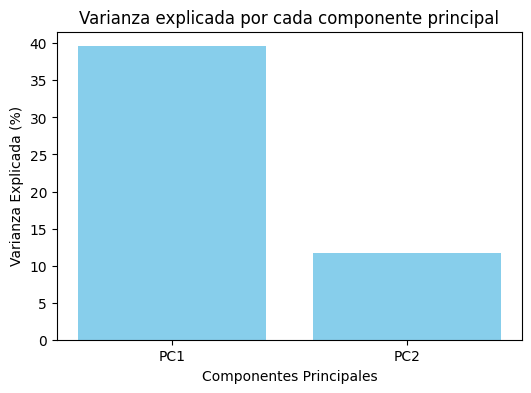
\includegraphics[scale = 0.75]{Enrique/Imagenes/Varianza_2d.png}
    \caption{Varianza de 51.32\%}
\end{figure}

\begin{figure}[!ht]
    \centering
    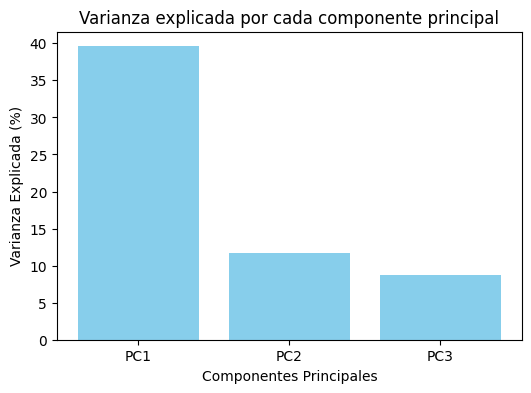
\includegraphics[scale = 0.75]{Enrique/Imagenes/varianza_3d.png}
    \caption{Varianza de 60.09\%}
\end{figure}

\subsubsection{Agrupamiento con DBSCAN}

También implementaremos el agrupamiento con el método \textit{DBSCAN}. Los primeros valores que proponemos para $\varepsilon$ y el número mínimo de muestras son 0.5 y 20 respectivamente, de lo cual obtenemos.

\begin{lstlisting}[caption={DSCAN con $\varepsilon$=0.5}]
    from sklearn.cluster import DBSCAN

    dbscan = DBSCAN(eps=.5, min_samples=20)
    dbscan.fit(scaled_data)

    print(dbscan.labels_.min(), dbscan.labels_.max())
\end{lstlisting}

\begin{lstlisting}[caption={Salida del código}]
    -1  9 
\end{lstlisting}

El -1 nos indica que el algoritmo clasificó algunos datos como \textit{atípicos}, que la etiqueta más grande sea 9 quiere decir que el algoritmo formó 10 grupos, como solo queremos formar 3 grupos, correremos el algoritmo para distintos valores de $\varepsilon$ hasta que solo se formen 3 \textit{clústeres}.

\begin{lstlisting}
    i = 0.5
    
    while dbscan.labels_.max() > 2:
        i += 0.1
        dbscan = DBSCAN(eps=i, min_samples=20)
        dbscan.fit(scaled_data)
        print(i, dbscan.labels_.min(), dbscan.labels_.max())
\end{lstlisting}

Con esto encontramos que la $\varepsilon$ que nos permite tener 3 grupos es 4.7, pero el algoritmo sigue clasificando algunos datos como atípicos, por lo que De manera similar encontramos el número de puntos mínimos

\begin{lstlisting}
    j = 20
    
    while dbscan.labels_.min() < 0 :
        j -= 1
        dbscan = DBSCAN(eps=4.9, min_samples=j)
        dbscan.fit(scaled_data)
        print(j, dbscan.labels_.min(), dbscan.labels_.max())
\end{lstlisting}

Finalmente obtenemos que $\varepsilon  =4.9$ y \textit{min\_samples = 19}, por lo que utilizaremos estos parámetros para el método \textit{DBSCAN}. Las etiquetas que obtengamos las guardaremos en una columna del \textit{dataframe scaled\_data\_df}

\begin{lstlisting}
    dbscan = DBSCAN(eps=4.9, min_samples=19)
    dbscan.fit(scaled_data)

    scaled_data_df['cluster DBSCAN'] = dbscan.labels_
\end{lstlisting}

    \subsection{Metodología de agrupamiento}
        Para trabajar con el problema de agrupamiento se utilizó el \textit{datset} ``Lung Cancer Prediction'', que puede consultarse en la página de Kaggle. Dicho \textit{dataset} tiene  mil registros de pacientes con cáncer de pulmón, cuenta con  25 características, entre las que se encuentran; edad, género, contaminación del aire, riesgo genético, dolor de pecho y el nivel de su condición (bajo, medio y alto). Si bien esta última característica podría permitirnos considerar a los datos como etiquetados, no la tomaremos en cuenta para poder trabajarlos con métodos de aprendizaje no supervisado. 

Las versiones de \textit{Python} y las librerías utilizadas fueron las siguientes:
\begin{itemize}
	\item  Pandas versión: 2.2.2
	
	\item  NumPy versión: 2.0.2
	
	\item  Seaborn versión: 0.13.2
	
	\item  Matplotlib versión: 3.10.0
	
	\item Sklearn versión: 1.6.1
	
	\item SciPy versión: 1.14.1
\end{itemize}

Como ya se mencionó, los registros tienen la característica \textit{'Level'}, por lo que el objetivo de esta sección es implementar métodos de agrupamiento para generar 3 \textit{clústeres} que nos permitan agrupar nuestros de manera similar a la característica \textit{'Level'}, debido a esto utilizaremos métodos de no jerárquicos, posteriormente utilizaremos el método \textit{PCA} para reducir la dimensión de nuestra \textit{dataset} para poder visualizar los \textit{clústeres} generados en gráficos 2D y 3D, finalmente compararemos los resultados que obtuvimos del agrupamiento con los datos originales para conocer la precisión que obtuvimos.

Primero hacemos una copia del \textit{dataset} con el que estamos trabajando y eliminamos las características \textit{'index', 'Patient ID'} y \textit{'Level'}, pues las primeras dos no son relevantes para el agrupamiento y ya planteamos que la última la usaremos para conocer la precisión que obtuvimos.

\subsubsection{Agrupamiento con k-means}

\lstset{
    language=Python,
    basicstyle=\ttfamily\footnotesize,
    keywordstyle=\color{blue},
    commentstyle=\color{gray},
    stringstyle=\color{green!60!black},
    numberstyle=\tiny\color{gray},
    numbers=left,
    breaklines=true,
    frame=single,
    captionpos=b,
    tabsize=4,
    showspaces=false,
    showstringspaces=false,
    showtabs=false
}
		
\begin{lstlisting}
    cancer_data = df.drop(columns=["Patient Id", "Level", "index"])

    # Estandarizamos los datos 
    scaler = StandardScaler()
    scaled_data = scaler.fit_transform(cancer_data)

    # Los convertimos en una data frame
    scaled_data_df = pd.DataFrame(scaled_data, columns=cancer_data.columns)
\end{lstlisting}

\begin{lstlisting}[caption={Código de k-means}]
    # posibles grupos: Low, Medium y High
    kmeans = KMeans(n_clusters=3, random_state=42, n_init=10)
    kmeans.fit(scaled_data)

    scaled_data_df['cluster'] = kmeans.labels_
\end{lstlisting}

Hacemos una reducción de dimensiones para poder visualizar los datos en 2D y 3D.  

\begin{lstlisting}[caption={PCA para 2D}]
    pca = PCA(n_components=2)
    cancer_pca = pca.fit_transform(scaled_data)
    print(f"Varianza total explicada: {sum(pca.explained_variance_ratio_)*100:.2f}%")
\end{lstlisting}

\begin{lstlisting}[caption={PCA para 3D}]
    pca3 = PCA(n_components=3)
    cancer_pca3 = pca.fit_transform(scaled_data)
    print(f"Varianza total explicada: {sum(pca3.explained_variance_ratio_)*100:.2f}%")
\end{lstlisting}

\begin{figure}[!ht]
    \centering
    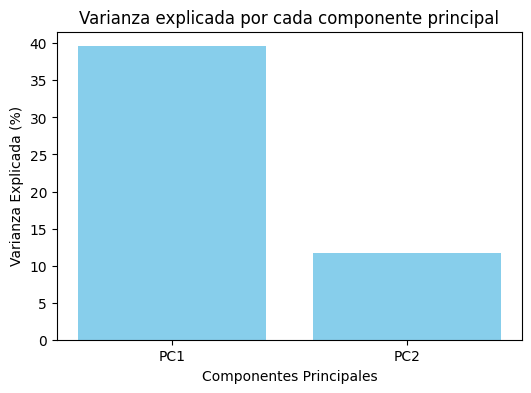
\includegraphics[scale = 0.75]{Enrique/Imagenes/Varianza_2d.png}
    \caption{Varianza de 51.32\%}
\end{figure}

\begin{figure}[!ht]
    \centering
    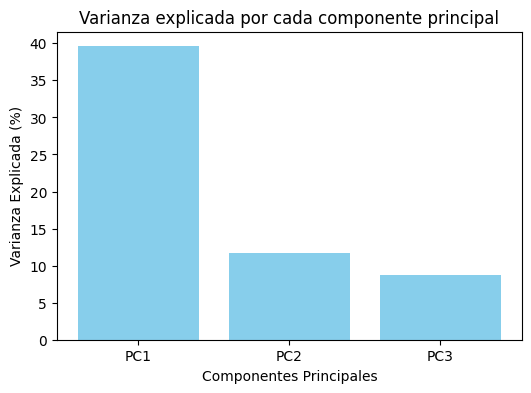
\includegraphics[scale = 0.75]{Enrique/Imagenes/varianza_3d.png}
    \caption{Varianza de 60.09\%}
\end{figure}

\subsubsection{Agrupamiento con DBSCAN}

También implementaremos el agrupamiento con el método \textit{DBSCAN}. Los primeros valores que proponemos para $\varepsilon$ y el número mínimo de muestras son 0.5 y 20 respectivamente, de lo cual obtenemos.

\begin{lstlisting}[caption={DSCAN con $\varepsilon$=0.5}]
    from sklearn.cluster import DBSCAN

    dbscan = DBSCAN(eps=.5, min_samples=20)
    dbscan.fit(scaled_data)

    print(dbscan.labels_.min(), dbscan.labels_.max())
\end{lstlisting}

\begin{lstlisting}[caption={Salida del código}]
    -1  9 
\end{lstlisting}

El -1 nos indica que el algoritmo clasificó algunos datos como \textit{atípicos}, que la etiqueta más grande sea 9 quiere decir que el algoritmo formó 10 grupos, como solo queremos formar 3 grupos, correremos el algoritmo para distintos valores de $\varepsilon$ hasta que solo se formen 3 \textit{clústeres}.

\begin{lstlisting}
    i = 0.5
    
    while dbscan.labels_.max() > 2:
        i += 0.1
        dbscan = DBSCAN(eps=i, min_samples=20)
        dbscan.fit(scaled_data)
        print(i, dbscan.labels_.min(), dbscan.labels_.max())
\end{lstlisting}

Con esto encontramos que la $\varepsilon$ que nos permite tener 3 grupos es 4.7, pero el algoritmo sigue clasificando algunos datos como atípicos, por lo que De manera similar encontramos el número de puntos mínimos

\begin{lstlisting}
    j = 20
    
    while dbscan.labels_.min() < 0 :
        j -= 1
        dbscan = DBSCAN(eps=4.9, min_samples=j)
        dbscan.fit(scaled_data)
        print(j, dbscan.labels_.min(), dbscan.labels_.max())
\end{lstlisting}

Finalmente obtenemos que $\varepsilon  =4.9$ y \textit{min\_samples = 19}, por lo que utilizaremos estos parámetros para el método \textit{DBSCAN}. Las etiquetas que obtengamos las guardaremos en una columna del \textit{dataframe scaled\_data\_df}

\begin{lstlisting}
    dbscan = DBSCAN(eps=4.9, min_samples=19)
    dbscan.fit(scaled_data)

    scaled_data_df['cluster DBSCAN'] = dbscan.labels_
\end{lstlisting}

\section{Resultados}

    \subsection{Resultados de clasificación}
        El fin de trabajar con dos modelos, el de regresión lineal y la red neuronal, es para comparar su desempeño y así mismo, sus respectivos resultados. Cabe destacar que el año ``objetivo'' es el 2040.

\subsubsection{Modelo de Regresión Lineal}

De manera concisa, el número total de muertes estimadas para el año 2040 por el Modelo de Regresión Lineal son: \textbf{10461.07}, proporcionándonos el siguiente gráfico: 

\begin{figure}[H] \centering 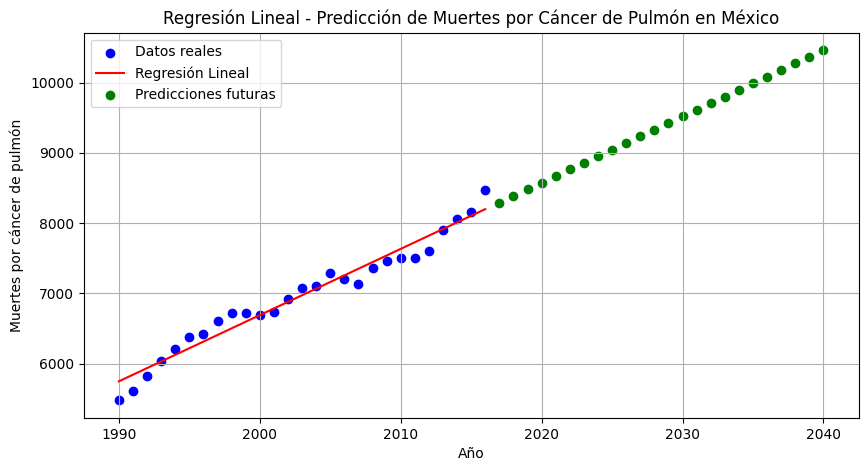
\includegraphics[width=0.70\textwidth]{Zdenko/Imágenes/regresion.png} \caption{Modelo de Regresión Lineal} \label{fig:regresion} \end{figure}

Como se puede apreciar, la evolución es completamente lineal.

\subsubsection{Red Neuronal Recurrente (LTSM)}

Por parte de la red neuronal concurrente, su predicción es de \textbf{7815.07}, arrojándonos el siguiente gráfico: 

\begin{figure}[h] \centering 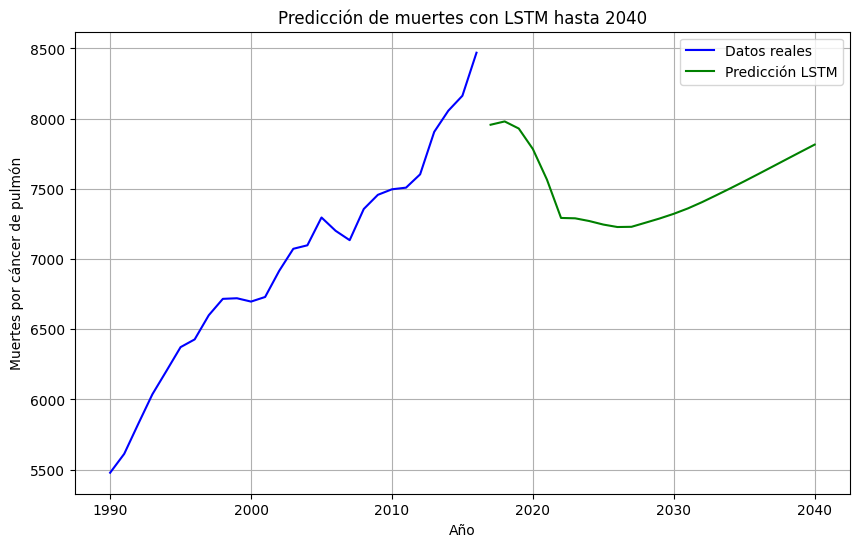
\includegraphics[width=0.85\textwidth]{Zdenko/Imágenes/red.png} \caption{Modelo LSTM} \label{fig:red} \end{figure}

A diferencia del modelo de regresión lineal, la red neuronal LSTM muestra un comportamiento menos lineal, adaptándose al conjunto de datos estudiados. 

\subsubsection{Comparación entre modelos}

Existe cierta cantidad de cálculo para la comparación entre diversos modelos, tales son: Error Absoluto Medio (MAE, por sus siglas en inglés), Error Cuadrático Medio (MSE, por sus siglas en inglés), Coeficiente de Determinación (R²); no obstante, en esta ocasión, solo nos centraremos en el MSE para realizar la comparación de desempeño y resultados entre ambos modelos.

\begin{figure}[H] 
    \centering 
    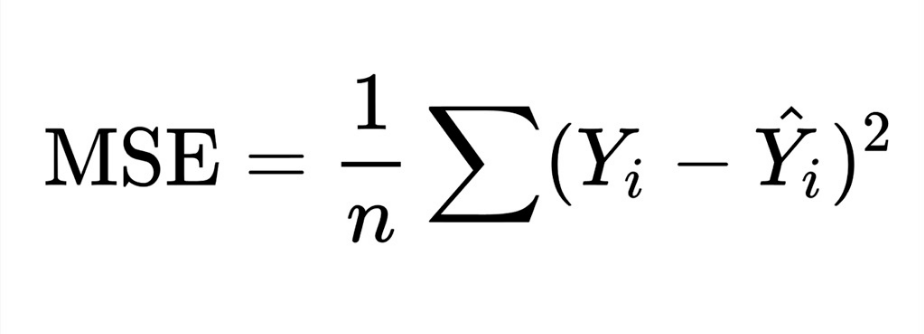
\includegraphics[width=0.5\textwidth]{Zdenko/Imágenes/formula_MSE.png} 
    \caption{Fórmula MSE} 
    \label{fig:formula} 
\end{figure}


El porqué radica en que en general, un MSE más bajo indica que el modelo está haciendo predicciones más precisas, ya que el error cuadrático castiga los errores grandes, lo que impulsa a los modelos a evitar grandes desviaciones. Es particularmente útil cuando deseas evitar errores muy grandes en las predicciones, como es el caso con las muertes causadas por cáncer de pulmón, donde un error grande podría tener consecuencias graves.

En este momento, estamos enfocados en observar qué modelo cuenta con un MSE menor. 

El cálculo del MSE tanto en el modelo de regresión lineal y la red neuronal LSTM fue realizado con la librería sklearn.metrics, haciendo uso de su método: "mean squared error".

\lstset{
    language=Python, % Define el lenguaje
    basicstyle=\ttfamily, % Configura la fuente del texto
    keywordstyle=\color{blue}, % Resalta las palabras clave en azul
    commentstyle=\color{green}, % Comentarios en verde
    stringstyle=\color{red}, % Cadenas de texto en rojo
    breaklines=true, % Permite saltos de línea en el código
}

\begin{lstlisting}
mse = mean_squared_error(y_test, y_pred)
\end{lstlisting}

\newpage

Por parte de la red neuronal, primero se desnormalizaron las predicciones para estar dentro del mismo rango de valores y posterior a eso, se aplicó el método de la librería: 

\lstset{
    language=Python,
    basicstyle=\ttfamily\footnotesize,
    keywordstyle=\color{blue},
    commentstyle=\color{gray},
    stringstyle=\color{green!60!black},
    numberstyle=\tiny\color{gray},
    numbers=left,
    breaklines=true,
    frame=single,
    captionpos=b,
    tabsize=4,
    showspaces=false,
    showstringspaces=false,
    showtabs=false
}

\begin{lstlisting}
# Hacer predicciones con el modelo LSTM en el conjunto de prueba
y_pred_lstm = model.predict(X_test)

# Desnormalizar las predicciones de la LSTM
y_pred_lstm_original = scaler_y.inverse_transform(y_pred_lstm)
y_test_original = scaler_y.inverse_transform(y_test)

# Calcular MSE con valores originales
mse_lstm = mean_squared_error(y_test_original, y_pred_lstm_original)
\end{lstlisting}

Dichos cálculos fueron útiles para realizar un gráfico y comparar sus resultados.
\begin{figure}[H] \centering 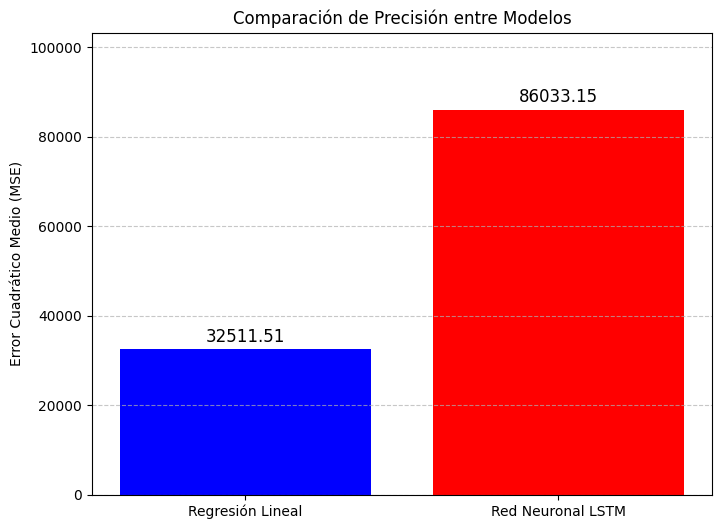
\includegraphics[width=0.75\textwidth]{Zdenko/Imágenes/comparacion.png} \caption{MSE en ambos modelos} \label{fig:comparacion} \end{figure}

Señalando que el modelo de regresión lineal, es más apropiado para este caso. 

    \subsection{Resultados de predicción}
        El fin de trabajar con dos modelos, el de regresión lineal y la red neuronal, es para comparar su desempeño y así mismo, sus respectivos resultados. Cabe destacar que el año ``objetivo'' es el 2040.

\subsubsection{Modelo de Regresión Lineal}

De manera concisa, el número total de muertes estimadas para el año 2040 por el Modelo de Regresión Lineal son: \textbf{10461.07}, proporcionándonos el siguiente gráfico: 

\begin{figure}[H] \centering 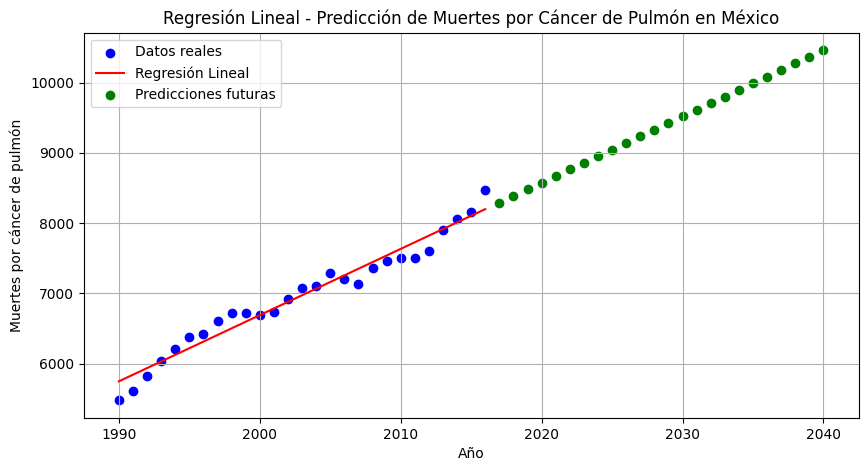
\includegraphics[width=0.70\textwidth]{Zdenko/Imágenes/regresion.png} \caption{Modelo de Regresión Lineal} \label{fig:regresion} \end{figure}

Como se puede apreciar, la evolución es completamente lineal.

\subsubsection{Red Neuronal Recurrente (LTSM)}

Por parte de la red neuronal concurrente, su predicción es de \textbf{7815.07}, arrojándonos el siguiente gráfico: 

\begin{figure}[h] \centering 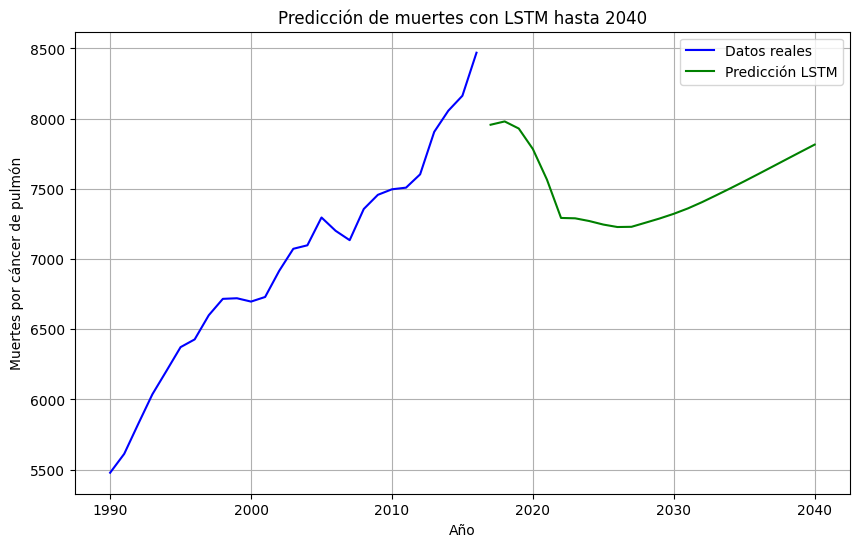
\includegraphics[width=0.85\textwidth]{Zdenko/Imágenes/red.png} \caption{Modelo LSTM} \label{fig:red} \end{figure}

A diferencia del modelo de regresión lineal, la red neuronal LSTM muestra un comportamiento menos lineal, adaptándose al conjunto de datos estudiados. 

\subsubsection{Comparación entre modelos}

Existe cierta cantidad de cálculo para la comparación entre diversos modelos, tales son: Error Absoluto Medio (MAE, por sus siglas en inglés), Error Cuadrático Medio (MSE, por sus siglas en inglés), Coeficiente de Determinación (R²); no obstante, en esta ocasión, solo nos centraremos en el MSE para realizar la comparación de desempeño y resultados entre ambos modelos.

\begin{figure}[H] 
    \centering 
    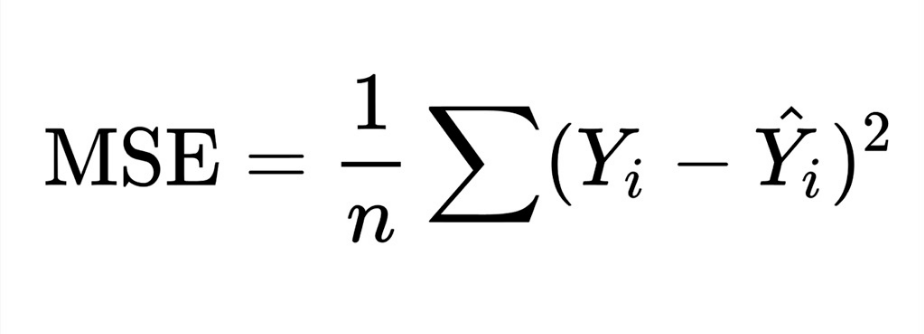
\includegraphics[width=0.5\textwidth]{Zdenko/Imágenes/formula_MSE.png} 
    \caption{Fórmula MSE} 
    \label{fig:formula} 
\end{figure}


El porqué radica en que en general, un MSE más bajo indica que el modelo está haciendo predicciones más precisas, ya que el error cuadrático castiga los errores grandes, lo que impulsa a los modelos a evitar grandes desviaciones. Es particularmente útil cuando deseas evitar errores muy grandes en las predicciones, como es el caso con las muertes causadas por cáncer de pulmón, donde un error grande podría tener consecuencias graves.

En este momento, estamos enfocados en observar qué modelo cuenta con un MSE menor. 

El cálculo del MSE tanto en el modelo de regresión lineal y la red neuronal LSTM fue realizado con la librería sklearn.metrics, haciendo uso de su método: "mean squared error".

\lstset{
    language=Python, % Define el lenguaje
    basicstyle=\ttfamily, % Configura la fuente del texto
    keywordstyle=\color{blue}, % Resalta las palabras clave en azul
    commentstyle=\color{green}, % Comentarios en verde
    stringstyle=\color{red}, % Cadenas de texto en rojo
    breaklines=true, % Permite saltos de línea en el código
}

\begin{lstlisting}
mse = mean_squared_error(y_test, y_pred)
\end{lstlisting}

\newpage

Por parte de la red neuronal, primero se desnormalizaron las predicciones para estar dentro del mismo rango de valores y posterior a eso, se aplicó el método de la librería: 

\lstset{
    language=Python,
    basicstyle=\ttfamily\footnotesize,
    keywordstyle=\color{blue},
    commentstyle=\color{gray},
    stringstyle=\color{green!60!black},
    numberstyle=\tiny\color{gray},
    numbers=left,
    breaklines=true,
    frame=single,
    captionpos=b,
    tabsize=4,
    showspaces=false,
    showstringspaces=false,
    showtabs=false
}

\begin{lstlisting}
# Hacer predicciones con el modelo LSTM en el conjunto de prueba
y_pred_lstm = model.predict(X_test)

# Desnormalizar las predicciones de la LSTM
y_pred_lstm_original = scaler_y.inverse_transform(y_pred_lstm)
y_test_original = scaler_y.inverse_transform(y_test)

# Calcular MSE con valores originales
mse_lstm = mean_squared_error(y_test_original, y_pred_lstm_original)
\end{lstlisting}

Dichos cálculos fueron útiles para realizar un gráfico y comparar sus resultados.
\begin{figure}[H] \centering 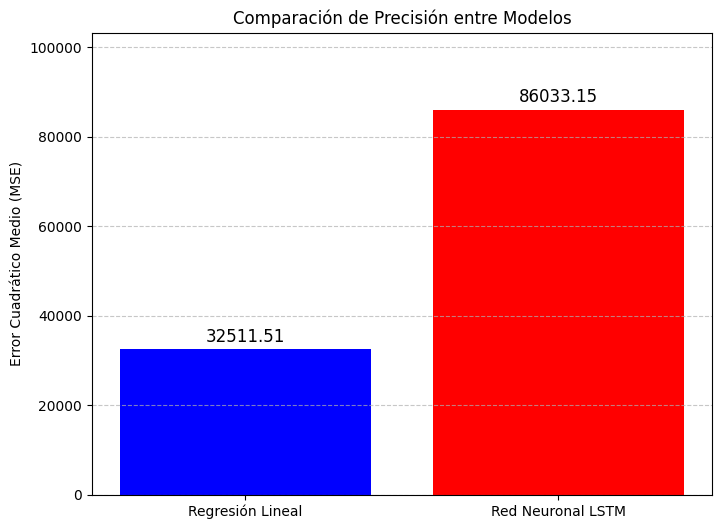
\includegraphics[width=0.75\textwidth]{Zdenko/Imágenes/comparacion.png} \caption{MSE en ambos modelos} \label{fig:comparacion} \end{figure}

Señalando que el modelo de regresión lineal, es más apropiado para este caso. 

    \newpage

    \subsection{Resultados de agrupamiento}
        El fin de trabajar con dos modelos, el de regresión lineal y la red neuronal, es para comparar su desempeño y así mismo, sus respectivos resultados. Cabe destacar que el año ``objetivo'' es el 2040.

\subsubsection{Modelo de Regresión Lineal}

De manera concisa, el número total de muertes estimadas para el año 2040 por el Modelo de Regresión Lineal son: \textbf{10461.07}, proporcionándonos el siguiente gráfico: 

\begin{figure}[H] \centering 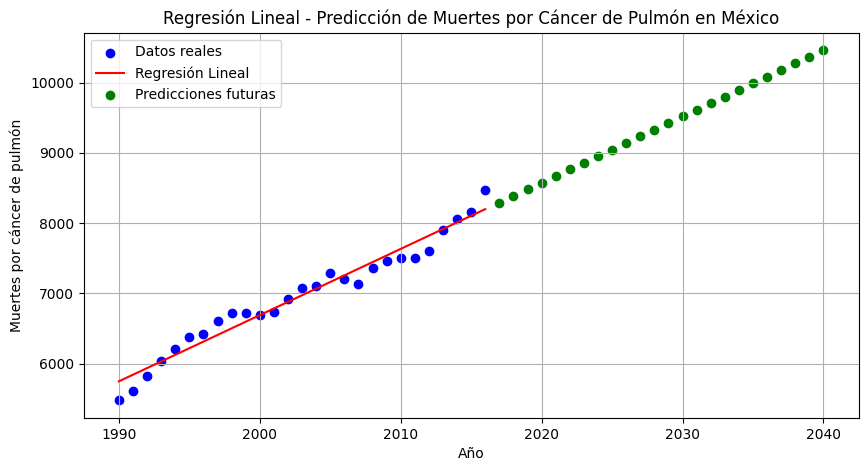
\includegraphics[width=0.70\textwidth]{Zdenko/Imágenes/regresion.png} \caption{Modelo de Regresión Lineal} \label{fig:regresion} \end{figure}

Como se puede apreciar, la evolución es completamente lineal.

\subsubsection{Red Neuronal Recurrente (LTSM)}

Por parte de la red neuronal concurrente, su predicción es de \textbf{7815.07}, arrojándonos el siguiente gráfico: 

\begin{figure}[h] \centering 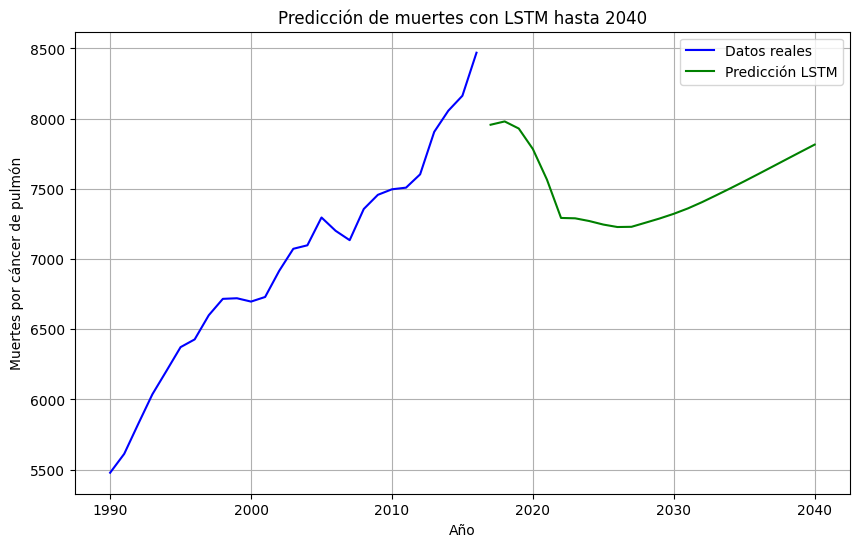
\includegraphics[width=0.85\textwidth]{Zdenko/Imágenes/red.png} \caption{Modelo LSTM} \label{fig:red} \end{figure}

A diferencia del modelo de regresión lineal, la red neuronal LSTM muestra un comportamiento menos lineal, adaptándose al conjunto de datos estudiados. 

\subsubsection{Comparación entre modelos}

Existe cierta cantidad de cálculo para la comparación entre diversos modelos, tales son: Error Absoluto Medio (MAE, por sus siglas en inglés), Error Cuadrático Medio (MSE, por sus siglas en inglés), Coeficiente de Determinación (R²); no obstante, en esta ocasión, solo nos centraremos en el MSE para realizar la comparación de desempeño y resultados entre ambos modelos.

\begin{figure}[H] 
    \centering 
    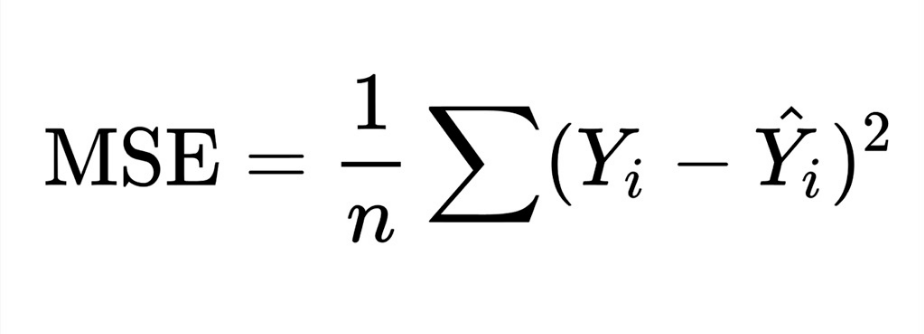
\includegraphics[width=0.5\textwidth]{Zdenko/Imágenes/formula_MSE.png} 
    \caption{Fórmula MSE} 
    \label{fig:formula} 
\end{figure}


El porqué radica en que en general, un MSE más bajo indica que el modelo está haciendo predicciones más precisas, ya que el error cuadrático castiga los errores grandes, lo que impulsa a los modelos a evitar grandes desviaciones. Es particularmente útil cuando deseas evitar errores muy grandes en las predicciones, como es el caso con las muertes causadas por cáncer de pulmón, donde un error grande podría tener consecuencias graves.

En este momento, estamos enfocados en observar qué modelo cuenta con un MSE menor. 

El cálculo del MSE tanto en el modelo de regresión lineal y la red neuronal LSTM fue realizado con la librería sklearn.metrics, haciendo uso de su método: "mean squared error".

\lstset{
    language=Python, % Define el lenguaje
    basicstyle=\ttfamily, % Configura la fuente del texto
    keywordstyle=\color{blue}, % Resalta las palabras clave en azul
    commentstyle=\color{green}, % Comentarios en verde
    stringstyle=\color{red}, % Cadenas de texto en rojo
    breaklines=true, % Permite saltos de línea en el código
}

\begin{lstlisting}
mse = mean_squared_error(y_test, y_pred)
\end{lstlisting}

\newpage

Por parte de la red neuronal, primero se desnormalizaron las predicciones para estar dentro del mismo rango de valores y posterior a eso, se aplicó el método de la librería: 

\lstset{
    language=Python,
    basicstyle=\ttfamily\footnotesize,
    keywordstyle=\color{blue},
    commentstyle=\color{gray},
    stringstyle=\color{green!60!black},
    numberstyle=\tiny\color{gray},
    numbers=left,
    breaklines=true,
    frame=single,
    captionpos=b,
    tabsize=4,
    showspaces=false,
    showstringspaces=false,
    showtabs=false
}

\begin{lstlisting}
# Hacer predicciones con el modelo LSTM en el conjunto de prueba
y_pred_lstm = model.predict(X_test)

# Desnormalizar las predicciones de la LSTM
y_pred_lstm_original = scaler_y.inverse_transform(y_pred_lstm)
y_test_original = scaler_y.inverse_transform(y_test)

# Calcular MSE con valores originales
mse_lstm = mean_squared_error(y_test_original, y_pred_lstm_original)
\end{lstlisting}

Dichos cálculos fueron útiles para realizar un gráfico y comparar sus resultados.
\begin{figure}[H] \centering 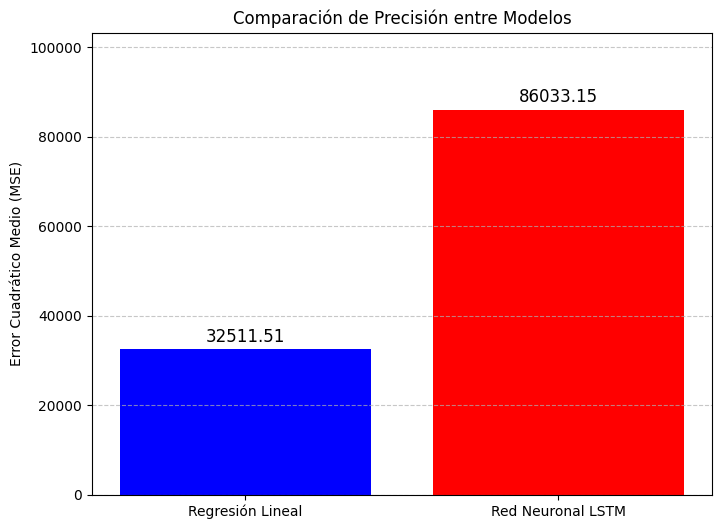
\includegraphics[width=0.75\textwidth]{Zdenko/Imágenes/comparacion.png} \caption{MSE en ambos modelos} \label{fig:comparacion} \end{figure}

Señalando que el modelo de regresión lineal, es más apropiado para este caso. 

\section{Conclusiones}

        Durante la investigación que se realizó para este trabajo se encontraron diversos artículos en los cuales se mencionan algunas de las principales causas del cáncer del pulmón, aunque algunos mencionan información relevante, como el factor de riesgo que presentan el alcohol y el tabaco también encontramos información sobre cáncer de pulmón en personas que jamás han fumado. Esta diversidad en las causas que se discuten nos llevo a aplicar los métodos aprendimos en el \textit{Samsung Innovation Campus} para averiguar si podíamos agrupar a los pacientes en base al nivel de su enfermedad con las características recopiladas.

En la sección de resultados podemos apreciar que nuestro objetivo no es posible, al menos con los datos y técnicas que trabajamos, en la matriz de confusión y el reporte de clasificación para \textit{DBSCAN} se aprecia que el modelo clasifica casi a todos los pacientes con un nivel bajo de la enfermedad lo cual ocasiona que tenga una precisión sumamente baja (36\%). 

Si bien, para el modelo de agrupamiento con \textit{k-means} se observa una mejoría significativa, sigue sin ser adecuada, pues en particular el modelo agrupa de manera muy pobre a los pacientes con un nivel alto de cáncer de pulmón, y esto es un elemento de suma importancia, además de que el agrupamiento para los pacientes con niveles bajos y medios de cáncer tampoco es lo suficientemente preciso. Aunque se podría considerar que el modelo tiene cierta utilidad, puesto que el recall para el nivel \textit{Low} fue de 76\% lo que nos indica que el 76\% de los pacientes que tienen un nivelo bajo de cáncer de pulmón fueron correctamente clasificados, esto sigue estando lejos de una precisión aceptable, y en lo general, la precisión del agrupamiento con \textit{k-means} (67\%) nos permite descartarlo. 

        El cáncer de pulmón representa un reto crítico para la salud pública tanto en México como a nivel mundial. Aunque en México ocupa el séptimo lugar en cuanto a frecuencia, se le reconoce como el tumor más letal, siendo la principal causa de muerte por cáncer. De acuerdo con el Dr. Omar Macedo Pérez, oncólogo del Instituto Nacional de Cancerología (INCan), anualmente fallecen cerca de ocho mil mexicanos por esta enfermedad, y se registran alrededor de nueve mil casos nuevos, de los cuales el 85\% están relacionados con el consumo de tabaco.

Este panorama se refleja también a nivel internacional. En la última década, la incidencia del cáncer de pulmón ha incrementado en un 30\%, con más de 2 millones de casos nuevos estimados tan solo en el año 2020 y alrededor de 1.8 millones de muertes. Si esta tendencia continúa, se espera que para el año 2030 se reporten más de 2.7 millones de casos nuevos anualmente. Estas cifras posicionan al cáncer de pulmón como una de las enfermedades oncológicas más agresivas y demandantes de atención prioritaria.

En el contexto mexicano, según datos recientes, en 2020 se registraron 7,811 nuevos casos y 6,733 muertes atribuibles a esta enfermedad. Tales datos refuerzan la relevancia del presente trabajo y la necesidad de contar con herramientas predictivas precisas que permitan anticipar el comportamiento de esta enfermedad en el futuro.

A partir del desarrollo de este proyecto y con base en la metodología aplicada para los modelos de predicción ---específicamente, la regresión lineal y la red neuronal recurrente (LSTM)--- se puede afirmar que los resultados obtenidos son coherentes con las estadísticas actuales. Las predicciones realizadas por ambos modelos se aproximan significativamente a las cifras reales reportadas en el país, lo que respalda su utilidad y validez para escenarios futuros.

\begin{enumerate}
    \item La evolución de las muertes por cáncer de pulmón en México sigue una tendencia lineal ascendente, reflejando un incremento sostenido año tras año. Esta tendencia podría agravarse en el futuro debido al creciente consumo de productos alternativos que contienen nicotina, como los vapeadores electrónicos y los sobres de nicotina (snus), los cuales representan un riesgo emergente para la salud pública.
    
    \item El modelo de regresión lineal mostró un buen desempeño en términos de precisión, aprovechando la estructura temporal de los datos disponibles. No obstante, al incrementar el volumen de datos y al incorporar variables adicionales relevantes ---como edad, género, comorbilidades, o hábitos de consumo---, las redes neuronales recurrentes podrían superar el rendimiento de los modelos tradicionales, al capturar patrones no lineales y relaciones más complejas en la evolución de la mortalidad.
\end{enumerate}

Estos hallazgos demuestran el potencial de las técnicas de aprendizaje automático y profundo como herramientas valiosas en el análisis epidemiológico y la toma de decisiones en salud pública. Su implementación puede contribuir significativamente al diseño de políticas preventivas y a la asignación más efectiva de recursos sanitarios en el país. \\ 

        Durante la investigación que se realizó para este trabajo se encontraron diversos artículos en los cuales se mencionan algunas de las principales causas del cáncer del pulmón, aunque algunos mencionan información relevante, como el factor de riesgo que presentan el alcohol y el tabaco también encontramos información sobre cáncer de pulmón en personas que jamás han fumado. Esta diversidad en las causas que se discuten nos llevo a aplicar los métodos aprendimos en el \textit{Samsung Innovation Campus} para averiguar si podíamos agrupar a los pacientes en base al nivel de su enfermedad con las características recopiladas.

En la sección de resultados podemos apreciar que nuestro objetivo no es posible, al menos con los datos y técnicas que trabajamos, en la matriz de confusión y el reporte de clasificación para \textit{DBSCAN} se aprecia que el modelo clasifica casi a todos los pacientes con un nivel bajo de la enfermedad lo cual ocasiona que tenga una precisión sumamente baja (36\%). 

Si bien, para el modelo de agrupamiento con \textit{k-means} se observa una mejoría significativa, sigue sin ser adecuada, pues en particular el modelo agrupa de manera muy pobre a los pacientes con un nivel alto de cáncer de pulmón, y esto es un elemento de suma importancia, además de que el agrupamiento para los pacientes con niveles bajos y medios de cáncer tampoco es lo suficientemente preciso. Aunque se podría considerar que el modelo tiene cierta utilidad, puesto que el recall para el nivel \textit{Low} fue de 76\% lo que nos indica que el 76\% de los pacientes que tienen un nivelo bajo de cáncer de pulmón fueron correctamente clasificados, esto sigue estando lejos de una precisión aceptable, y en lo general, la precisión del agrupamiento con \textit{k-means} (67\%) nos permite descartarlo. 
    
\newpage
\addcontentsline{toc}{section}{Referencias} % Para que aparezcan en el índice
\printbibliography

\end{document}
    